\documentclass[review]{elsarticle}

\usepackage{lineno,hyperref}
\modulolinenumbers[5]

\journal{Physica A}

%%%%%%%%%%%%%%%%%%%%%%%
%% Elsevier bibliography styles
%%%%%%%%%%%%%%%%%%%%%%%
%% To change the style, put a % in front of the second line of the current style and
%% remove the % from the second line of the style you would like to use.
%%%%%%%%%%%%%%%%%%%%%%%

%% Numbered
%\bibliographystyle{model1-num-names}

%% Numbered without titles
%\bibliographystyle{model1a-num-names}

%% Harvard
%\bibliographystyle{model2-names.bst}\biboptions{authoryear}

%% Vancouver numbered
%\usepackage{numcompress}\bibliographystyle{model3-num-names}

%% Vancouver name/year
%\usepackage{numcompress}\bibliographystyle{model4-names}\biboptions{authoryear}

%% APA style
%\bibliographystyle{model5-names}\biboptions{authoryear}

%% AMA style
%\usepackage{numcompress}\bibliographystyle{model6-num-names}

%% `Elsevier LaTeX' style
\bibliographystyle{elsarticle-num}
%%%%%%%%%%%%%%%%%%%%%%%

\begin{document}

\begin{frontmatter}

\title{Language differentiation in complex social interaction networks}
% OR
% \title{Language differentiation in the elementary sectors of complex social interaction networks}
% OR
% \title{Language differentiation in complex social networks}
% OR
% \title{Language differentiation in the Erdös sectors of complex social networks}
% \tnotetext[mytitlenote]{Fully documented templates are available in the elsarticle package on \href{http://www.ctan.org/tex-archive/macros/latex/contrib/elsarticle}{CTAN}.}

%% Group authors per affiliation:
\author[mainaddr]{Renato Fabbri\corref{mycorrespondingauthor}}
\cortext[mycorrespondingauthor]{Corresponding author}
\ead{fabbri@usp.br}

%% or include affiliations in footnotes:
\author[secaddr]{Osvaldo N. Oliveira Jr.}

\address[mainaddr]{Institute of Mathematics and Computer Sciences (ICMC/USP) - Avenida Trabalhador São-carlense, 400 - Centro, São Carlos, SP, Brazil}
  \address[secaddr]{São Carlos Institute of Physics (IFSC/USP) - Avenida Trabalhador São-carlense, 400 - Centro, São Carlos, 13566-590, SP, Brazil}

\begin{abstract}
  Social networks have been widely considered in recent scientific literature.
  A central question remains, though: how are the linguistic and topological features of
  social actors related?
  In this work, we demonstrate a fundamental association between sectors of networks
  and the language used therein.
  The hubs, intermediary and peripheral sectors of a network, defined though the
  connectivity distribution, exhibit statistical distances, between the texts they produce,
  often greater than between texts of different networks or even the same sectors of different networks.
  This result holds for networks related to very distinct subjects, such as programming libraries and
  national elections, and are valid for raw textual features (such as token size),
  gramatic features (such as fraction of adjectives), and semantic features
  (such as obtained through the canonical Wornet).
  The findings herein reported should assist further studies relating language and topology
  in social networks, e.g. by relating communities or special groups of agents, such as of brokers
   and those with a high clustering coefficient, and by the consideration of other social networking systems.
\end{abstract}

\begin{keyword}
social networks\sep complex letworks \sep language \sep text mining \sep Erdös sectors
\MSC[2019] 00-01\sep  99-00
\end{keyword}

\end{frontmatter}

\linenumbers

\section{Introduction}

\section{Materials and methods}
\subsection{Mining email lists}
Email list messages were obtained from
the Gmane email archive, which consists of more than $20,000$
email lists (discussion groups) and more than $130\times 10^6$ messages~\cite{GMANEwikipedia}. These lists cover a variety of topics, mostly technology-related. The archive can be described as a corpus along with message metadata, including sent time, place, sender name, and sender email address.
The usage of the Gmane database in scientific research is reported in studies of isolated lists and of lexical innovations~\cite{Gmane2,bird}. 

We observed various email lists and data from Twitter, Facebook and Participabr.
For a thorough analysis, we selected five of the email lists
from which general properties can be inferred.
These lists are as follows:

\begin{itemize}
\item Linux Audio Users list\footnote{gmane.linux.audio.users is list ID in Gmane.}, with participants from different countries with artistic and technological interests. English is the prevailing language. Abbreviated as LAU from now on.

\item Linux Audio Developers list\footnote{gmane.linux.audio.devel is list ID in Gmane.}, with participants from different countries; a more technical and less active version of LAU. English is the prevailing language. Abbreviated as LAD from now on.

\item Developer's list for the standard C++ library\footnote{gmane.comp.gcc.libstdc++.devel is list ID in Gmane.}, with computer programmers from different countries. English is the prevailing language. Abbreviated as CPP from now on.
\item List of the MetaReciclagem project\footnote{gmane.politics.organizations.metareciclagem is list ID in Gmane.}, a Brazilian email list for digital culture. Portuguese is the prevailing language, although some messages are written in Spanish and English. Abbreviated as MET from now on.
\item List for de discussion of the election reform\footnote{gmane.politics.election-methods is list ID in Gmane.}. English is the prevailing language. Abbreviated ELE from now on.
\end{itemize} 
We systematicaly used 18 lists for taking text-related metrics.


\begin{table}
\centering
\caption{Columns $date_1$ and $date_M$ have dates of first and last messages from the 20,000 messages considered in each email list.
$N$ is the number of participants (number of different email addresses),
$\Gamma$ is the number of discussion threads (count of messages without antecedent),
$\overline{M}$ is the number of messages missing in the 20,000 collection
($100\frac{23}{20000}=0.115$ percent in the worst case).
}
	\def\arraystretch{1.2}
\label{tab:genLists}
\begin{tabular}{l|c|c|c|c|c}\hline
list & $date_1$ & $date_{M}$ & $N$ & $\Gamma$ & $\overline{M}$ \\\hline
LAU & 2003-06-29  & 2005-07-23  & 1147  & 3374  & 5 \\
LAD & 2003-07-03  & 2009-10-07  & 1232  & 3114  & 4 \\
MET & 2005-08-01  & 2008-03-07  & 477  & 4607  & 23 \\
CPP & 2002-03-12  & 2009-08-25  & 1036  & 4506  & 7 \\
ELE & 2002-03-18  & 2011-08-31  & 302  & 6070  & 54 \\\hline

\end{tabular}
\begin{flushleft}\footnotesize
Source: By the author.\
\end{flushleft}
\end{table} 

\subsection{Interaction networks}
Edges in interaction networks can be modeled both as weighted or unweighted, as directed or undirected~\cite{bird,newmanCommunityDirected,newmanCommunity2013}.
Networks in this thesis are directed and weighted, the most informative of the possibilities. We did not investigate directed unweighted, undirected weighted, and undirected unweighted representations of the interaction networks. 

The interaction networks were obtained as follows: a direct response from participant B to a message from participant A yields an edge from A to B, as information went from A to B. The reasoning is: if B wrote a response to a message from A, he/she read what A wrote and formulated a response, so B assimilated information from A, thus $A \rightarrow B$.
Edges in both directions are allowed. Each time an interaction occurs, the value of one is added to the edge weight. Selfloops were regarded as non-informative and discarded. Inverting edge direction yields the status network: B read the message and considered what A wrote worth responding, giving status to A, thus $B\rightarrow A$. This thesis considers by convention the information network as described above ($A\rightarrow B$) and depicted in Figure~\ref{formationNetwork}. These interaction networks are reported in the literature as exhibiting scale-free and small-world properties, as expected for a number of social networks~\cite{bird,newmanBook}.

\begin{figure}[!h]
\centering
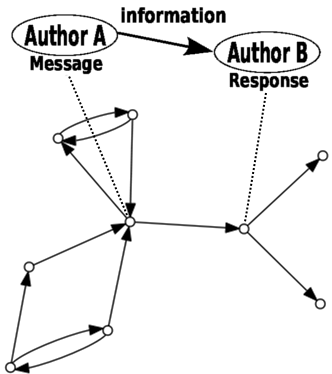
\includegraphics[width=0.5\textwidth]{figs/criaRede3_}
\caption{The formation of interaction networks from exchanged messages. Each vertex represents a participant. A reply message from author B to a message from author A is regarded as evidence that B received information from A and yields a directed edge. Multiple messages add ``weight'' to a directed edge. Further details are given in Section~\ref{intNet}.}
\label{formationNetwork}
\begin{flushleft}\footnotesize
Source: By the author.\
\end{flushleft}
\end{figure}


\subsection{Sectioning of a network into hub, intermediary and peripheral nodes (Erdös sectioning)}
It is often useful to think of vertices as hubs, peripheral and intermediary. We have therefore derived the peripheral, intermediary and hub sectors of an empirical network from the comparison against an Erd\"os-R\'enyi network with the same number of edges and vertices,
as depicted in Figure~\ref{fig:setores}. We refer to this procedure as \emph{Erd\"os sectioning}, with the resulting sectors being named as \emph{Erd\"os sectors}. The Erd\"os sectioning was recognized as a theoretical possibility by M. O. Jackson in his video lectures~\cite{3setores}, but to our knowledge it has not as yet been applied to empirical data.

The degree distribution $\widetilde{P}(k)$ of a real network with a scale-free profile $\mathcal{N}_f(N,z)$ with $N$ vertices and $z$ edges has less
average degree nodes than the distribution $P(k)$ of an Erd\"os-R\'enyi
network with the same number of vertices and edges. Indeed, we define in this work the intermediary sector of a network to be the set of all the nodes whose degree is less abundant in the real network than on the Erd\"os-R\'enyi model:

\begin{equation}\label{criterio}
\widetilde{P}(k)<P(k) \Rightarrow \text{k is intermediary degree}
\end{equation}

If $\mathcal{N}_f(N,z)$ is directed and has no self-loops, the probability of the existence
of an edge between two arbitrary vertices is $p_e=\frac{z}{N(N-1)}$.
A vertex in the ideal Erd\"os-R\'enyi digraph with the same number of vertices and edges, and thus the same probability $p_e$ for the presence of an edge, will have degree $k$ with probability

\begin{equation}
P(k)=\binom{2(N-1)}{k}p_e^k(1-p_e)^{2(N-1)-k}
\end{equation}

The lower degree fat tail corresponds to the border vertices, i.e. the peripheral sector or periphery where $\widetilde{P}(k)>P(k)$ and $k$ is lower than any value of $k$ in the intermediary sector.
The higher degree fat tail is the hubs sector, i.e. $\widetilde{P}(k)>P(k)$ and $k$ is higher than any value of $k$ in the intermediary sector. The reasoning for this classification is as follows: vertices so connected that they are virtually nonexistent in the Erd\"os-R\'enyi model, are coherently associated to the hubs sector.
Vertices with very few connections, which are way more abundant than expected in the Erd\"os-R\'enyi model,
are assigned to the periphery.
Vertices with degree values predicted as the most abundant in the Erd\"os-R\'enyi model,
near the average, and less frequent in the real network, are classified as intermediary.

\clearpage
\begin{figure}[!h]
\centering
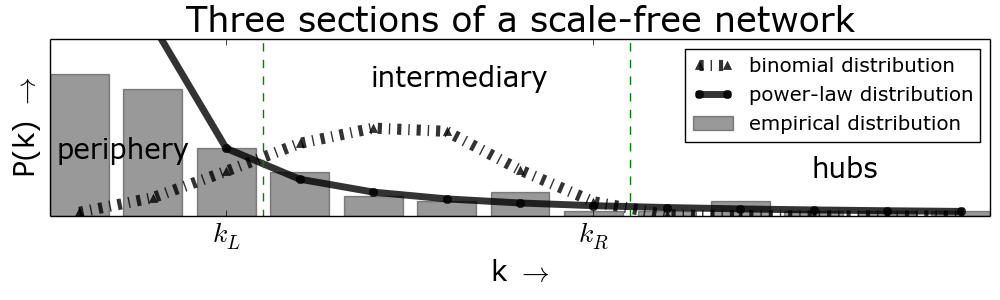
\includegraphics[width=\textwidth]{figs/fser__}
\caption{Classification of vertices by comparing degree
distributions~\cite{3setores}.
The binomial distribution of the Erd\"os-R\'enyi network model exhibits more intermediary vertices, while a scale-free network, associated with the power-law distribution, has more peripheral and hub vertices. The sector borders are defined with respect to the intersections of the distributions. Characteristic degrees are in the compact intervals: $[0,k_L]$, $(k_L,k_R]$, $(k_R,k_{max}]$ for the periphery, intermediary and hub sectors, the ``Erd\"os sectors''.
The connectivity distribution of empirical interaction networks, e.g. derived from email lists, can be sectioned by comparison against the associated binomial distribution with the same number of vertices and edges. In this figure, a snapshot of 1000 messages from CPP list yields the degree distribution of an interaction network of 98 nodes and 235 edges. A thorough explanation of the method is provided in Section~\ref{sectioning}.}
\label{fig:setores}
\begin{flushleft}\footnotesize
Source: By the author.\
\end{flushleft}
\end{figure}

\subsection{Text-related measures}
This work focuses on very simple metrics derived from texts as they have been sufficient for current interests.
Such metrics are:
\begin{itemize}
\item Frequency of characters: letters, vowels, punctuations and uppercase letters.
\item Number of tokens, frequency of punctuations among tokens, frequency of known words, frequency of words that have Wordnet synsets, frequency of tokens that are stopwords.
\item Mean and standard deviation for word, token sentence and message sizes.
\item Fraction of morphosyntactic classes, such as adverbs, adjectives, nouns and other POS (Part-Of-Speech) tags.
	We implemented a Brill POS tagger because of the massive amount of textual data that we had to analyze (the Brill tagger is very fast).
	We used the ``universal'' tagset described in~\cite{petrov} (developed to account for many languages) and trained the tagger with both Brown and Treebank corpus\footnote{We
		used the full Brown corpus while only 5\% of the Penn Treebank (as included in NLTK~\cite{trabNLTK}).}
	divided into 80/20\% of sentences for training and evaluation. The tagger achieved $94.95\%$ of accuracy.
\item Fraction of words in each Wordnet~\cite{wordnet} top-most hypernyms,
such as abstraction and physical entities for nouns or act for verbs.
\item Mean and standard deviation of the number of Wordnet synset relations, such as holonyms and meronyms, domains, lemmas and verb groups.
\end{itemize}
% \noindent To such metrics are dedicated Tables~\ref{tab:cha},~\ref{tab:tokens},~\ref{tab:sizesTokens},~\ref{tab:sizesSents},~\ref{tab:sizesMsgs},~\ref{tab:pos}.

This choice is based on: 1) the lack of such information in the literature, to the best of our knowledge; 
2) potential relations of these incidences with topological aspects, such as connectivity;
3) the interdependence of textual artifacts suggests that simple metrics should reflect complex and more subtle aspects.
A preliminary study, with the complete works from the Brazilian writer Machado de Assis~\cite{machado},
made clear that these metrics vary with respect to style.

\subsubsection{About Wordnet}
In this thesis, we made use of the statistics derived from the incidence of Wordnet synsets and their characteristics.
This calls for a brief description of what Wordnet is, what is a synset and what are such characteristics:
\begin{itemize}
\item Wordnet: a lexical database for the English language released in a BSD style license. It groups synonyms into synsets, provides a number of relations among the synsets, definitions and use examples.
\item Synset: defined by Wordnet documentation as a set of one or more synonyms that are (somewhat) interchangeable without changing the true value of the proposition in which they occur.
\item Synset characteristics: a synset is associated to other synsets by a number of semantic relations which differ with the POS tag attributed to them.
Examples of such relations include hyponyms and hypernyms (respectively less and more general terms), meronyms and holonyms (respectively is part of and has part), lemmas (canonical forms of a word), similar words by semantic criteria, entailments.
Some characteristics are derived from the synset in relation to the whole Wordnet network.
In this respect, we used only the maximum and minimum depth of the synset, which are respectively the maximum and minimum number of hypernyms from the synset to the root synset (e.g. 'thing' for nouns).
\end{itemize}

\subsubsection{Relating text and topology}\label{sec:ks}
The topological and textual metrics were related by:
\begin{enumerate}
\item textual metrics in hub, intermediary and peripheral network sectors, which are delimited by topological criteria as described in Section~\ref{sectioning}.
\item Correlation of metrics of each vertex, facilitating pattern detection involving topology of interaction and language.
\item Principal components formation derived from the usual Principal Component Analysis.
\end{enumerate}

\subsection{Statistical distances}
An adaptation of the Kolmogorov-Smirnov test was used to observe differences in textual content, as follows.
Let $F_{1,n}$ and $F_{2,n'}$ be two empirical distribution functions, where $n$ and $n'$ are the number of observations on each sample.
The two-sample Kolmogorov-Smirnov test rejects the null hypothesis (that the samples are drawn from the same underlying distribution) if:
\begin{equation}\label{eq:ks}
D_{n,n'} > c(\alpha)\sqrt{\frac{n+n'}{nn'}}
\end{equation}

\noindent where $D_{n,n'}=sup_x[F_{1,n}-F_{2,n'}]$ is the Kolmogorov-Smirnov statistic
and $c(\alpha)$ is related to the significance level $\alpha$ by:

\begin{table}[H]
\centering
\begin{tabular}{l||c|c|c|c|c|c}\hline
$\alpha$ & 0.1 & 0.05 & 0.025 & 0.01 & 0.005 & 0.001 \\
$c(\alpha)$ & 1.22 & 1.36 & 1.48 & 1.63 & 1.73 & 1.95 \\\hline
\end{tabular}
\begin{flushleft}\footnotesize
	Source: KOLMOGOROV-SMIRNOV test~\cite{kolm}.\
\end{flushleft}
\end{table}

We need to compare empirical distribution functions,
therefore $D_{n,n'}$ is given, as are $n$ and $n'$.
All terms in equation~\ref{eq:ks} are positive and $c(\alpha)$ can be isolated:

\begin{equation}\label{eq:ks2}
c(\alpha) < \frac{D_{n,n'}}{\sqrt{\frac{n+n'}{nn'}}} = c'
\end{equation}

When $c'$ is high, corresponding low values of $\alpha$ favor rejecting the null hypothesis.
For example, when $c'$ is greater than $\approx 1.7$, one might assume that $F_{1,n}$ and $F_{2,n'}$ differ.
We used $c'$ as a measure of how much
the distributions differ
and for deriving hypotheses
about how different are the underlying mechanisms of generation of texts.
We made systematic measurements of the $c'$ statistic in~\cite{kolmSmir}
which illustrate that $c'$ and $D_{n,n'}$ are useful in considering the
similarity or difference in the distributions underlying sets of observations.
A note of caution should be given here: what is a difference in distributions
might vary with context.
A $D_{n,n'}$ of only $0.0001$ will yield a very large $c'$ if $n$ and $n'$ are large enough.
On the other hand, a large $D_{n,n'}$ with a small $c'$ is not a strong evidence that
the distributions differ.
Therefore, we consider both $D_{n,n'}$ and $c'$ simultaneously in our analysis.

\section{Results and discussion}
The consideration of all measures and all distances results in a vast number of measurements, comparisons and tables.
Also, a thorough discussion of these outcomes becomes lengthy and tiresome.
We here present a summary of the findinds and
a more comprehensive presentation is available at~\cite{thesis} if
the reader finds necessary.

The most important result of is the strong statistical evidence of differentiation of each Erd\"os sector with respect to the language used.
This conclusion can be reached by observing the differences in the measurements of textual features in
each sector, and is supported on firm theoretical grounds by using the adapted Kolmogorov-Smirnov test presented in Section~\ref{sec:ks}.
% derived from the kolmogorov-smirnov test adaptation
Other relevant results are:
\begin{itemize}
\item the identification of patterns in the frequency of use of nouns, adverbs, sizes of words, depth of Wordnet synsets and other linguistic traces, by different types of participants in the Erd\"os sectors. We did not find in the literature any indication for such values; thus we believe it is useful to report e.g. that about 15\% of the characters are spaces and that nouns often account for more than 25\% of the words.
These values are available in~\cite{textTables} and not in the body of the text,
                since the focus here is the evidence that texts from distinct sectors differ.
\item Evidence of what is different in the texts produced by each Erd\"os sector. For example: hubs were found to use more contractions,
more common words, and less punctuation if compared to the rest of the network,
especially the peripheral sector.
In general, the rise or fall of a text-related metric is not relevant or is monotonic along connectivity,
but some of them reach extreme values in the intermediary sector.
\end{itemize}

The next sections summarize results of immediate interest
and further insights can be obtained by skimming through
the tables and figures of~\cite{stab,textTables} and the Conclusions chapter.
We illustrate with just one table of each kind,
and from networks obtained with 2000 messages.
In~\cite{textTables} we display tables for various networks.
In the same document, we relate the email lists to each numerical
TAG in the tables of the following sections.
The scale of 1000 and 2000 messages was chosen for deriving results,
as the networks in this scale are found to have stable topological structure,
as described in~\cite{stab}.
The findings with 1000 messages are the same as with 2000 messages,
and there are many tables.
This motivated the exclusion of the tables with measurements in
networks of 1000 messages.

\subsection{General characteristics of activity distribution among sectors}\label{sec:gen}
Before we dig into the findings derived from text-related measurements,
let us look once more at the general structure of these networks,
now giving emphasis on the activity of the sectors.
In almost all our observations,
the peripheral sector was responsible for starting most of the discussion threads,
i.e. for sending messages to the list which are not replies.
This is surprising since the peripheral sector is responsible for fewer messages. It suggests complementarity between peripheral diversity and hub specialization, which, on its turn, deepens the understanding of the interaction network as a meaningful system. 
These assertions are condensed in Table~\ref{geralListas}.
Less often, the intermediary sector is responsible for the largest number of messages and of threads.
Also meaningful is that the hubs sector is responsible for most of the messages, which is not obvious: hub participants are far more active but way less numerous. Interestingly, in such a setting where every characteristic differs with respect to
distinct sectors, there was no evidence of difference on the size of the threads started by each sector.
\begin{table}[h!]
\begin{center}
\begin{tabular}{| l || c | c | c | c |}\hline
 & {\bf g.} & {\bf p.} & {\bf i.} & {\bf h.} \\\hline\hline
$N$ & 17.00  & 7.00  & 6.00  & 4.00 \\
$N_{\%}$ & 100.00  & 41.18  & 35.29  & 23.53 \\\hline
$M$ & 100.00  & 11.00  & 37.00  & 52.00 \\
$M_{\%}$ & 100.00  & 11.00  & 37.00  & 52.00 \\\hline
$\Gamma$ & 18.00  & 4.00  & 8.00  & 6.00 \\
$\Gamma_{\%}$ & 100.00  & 22.22  & 44.44  & 33.33 \\\hline
$\frac{\Gamma}{M}\%$ & 18.00  & 36.36  & 21.62  & 11.54 \\
$\mu(\gamma)$ & 2.67  & 2.50  & 2.75  & 2.67 \\
$\sigma(\gamma)$ & 0.47  & 0.50  & 0.43  & 0.47 \\\hline
\end{tabular}
\caption{Distribution of participants, messages and threads among each Erd\"os sector ({\bf p.} for periphery, {\bf i.} for intermediary, 
    {\bf h.} for hubs) in a total time period of 0.71 years (from 2007-04-24T18:54:28 to 2008-01-10T19:17:26). $N$ is the number of participants, $M$ is the number of messages, $\Gamma$ is the number of threads, and $\gamma$ is the number of messages in a thread.
    The \% denotes the usual `per cent' with respecto to the total quantity ($100\%$ for {\bf g.})
    while $\mu$ and $\sigma$ denote mean and standard deviation.}
\end{center}
\end{table}

\subsection{Evidence that the texts from Erd\"os sectors differ}\label{subsec:di}
Results from our adaptation of the Kolmogorov-Smirnov test (see Section~\ref{sec:ks})
present strong evidence
that the text produced by each sector are different.
Tables~\ref{tab:kolTok}-\ref{tab:kolPctInter}
illustrate three results:
\begin{itemize}
 \item There is statistical evidence that the textual production of the Erd\"os sectors is different.
	 This can be noticed from the high values of $c'$ on these tables, clearly above reference values used for the acceptance of the null hypothesis (the null hypothesis being that the probability distributions generating the samples are the same). Also, we regarded as non-negligible the values often above 0.1 for the Kolmogorov-Smirnov statistics (the maximum difference between the cumulative distributions), which we recognized as relevant for assuming differences in the underlying distributions in our study (see Section~\ref{sec:ks}).
  \item Intermediary sectors sometimes exhibit greater differences 
from periphery and hubs than these extreme sectors between themselves 
(Tables~\ref{tab:kolTok} and~\ref{tab:kolSub}).
This differentiation of the three sectors is an indication that the Erd\"os Sectioning described in Section~\ref{sectioning} reveals meaningful sectors of the networks.
 \item The evidence of difference (as measured by $c'$) between sectors on the same network (Tables~\ref{tab:kolTok}-\ref{tab:kolPct}) is often larger than found between the same sector from distinct networks (Tables~\ref{tab:kolSubInter}-\ref{tab:kolPctInter}).
 \end{itemize}

 In Tables~\ref{tab:kolTok}-\ref{tab:kolPct}, there are two measurements for each pair of sectors.
 The top value is $c'$ while the bottom value is the Kolmogorov-Smirnov statistic.
 In Tables~\ref{tab:kolSubInter}-\ref{tab:kolPctInter} only $c'$ values are shown to illustrate
 that the measurements found between networks are comparable to measurements found between sectors of a same network.
 \begin{table}[h!]
\begin{center}
	\caption{Measurements of $c'$ and the KS statistic related to sizes of tokens between the Erd\"os sectors and the whole network. The abbreviations are: g for global, p for peripheral, i for intermediary, h for hubs. See Section~\ref{sec:ks} for and explanation of the measures and Section~\ref{subsec:di} for discussion. TAG of list: 6}
\label{tab:kolTok}
\begin{tabular}{l ? c c c | c c c}
{\bf } & {\bf p-g} & {\bf i-g} & {\bf h-g} & {\bf p-i} & {\bf p-h} & {\bf i-h} \\\hline
$c'$ & 4.327  & 17.168  & 7.851  & 18.907  & 7.833  & 15.540 \\
KS & 0.014  & 0.115  & 0.044  & 0.129  & 0.045  & 0.129 \\
\end{tabular}
\end{center}
\end{table}

 \begin{table}[h!]
\begin{center}
\caption{Measurements of $c'$ and the KS statistic related to sizes of known words between the Erd\"os sectors and the whole network. The abbreviations are: g for global, p for peripheral, i for intermediary, h for hubs. See Section~\ref{sec:ks} for and explanation of the measures and Section~\ref{subsec:di} for discussion. TAG of list: 1}
\begin{tabular}{l | c c c c c c}
{\bf } & {\bf p-g} & {\bf i-g} & {\bf h-g} & {\bf p-i} & {\bf p-h} & {\bf i-h} \\\hline
$c'$ & 5.904  & 5.264  & 5.549  & 9.547  & 7.073  & 4.058 \\
KS & 0.043  & 0.040  & 0.150  & 0.083  & 0.193  & 0.111 \\
\end{tabular}
\end{center}
\end{table}

 \begin{table}[h!]
\begin{center}
\caption{Measurements of $c'$ and the KS statistic related to sizes of sentences between the Erd\"os sectors and the whole network. The abbreviations are: g for global, p for peripheral, i for intermediary, h for hubs. See Section~\ref{sec:ks} for and explanation of the measures and Section~\ref{subsec:di} for discussion. TAG of list: 2}
\begin{tabular}{l ? c c c | c c c}
{\bf } & {\bf p-g} & {\bf i-g} & {\bf h-g} & {\bf p-i} & {\bf p-h} & {\bf i-h} \\\hline
$c'$ & 0.733  & 2.077  & 2.834  & 1.642  & 2.589  & 4.139 \\
KS & 0.020  & 0.038  & 0.059  & 0.048  & 0.080  & 0.097 \\
\end{tabular}
\end{center}
\end{table}


 \begin{table}[h!]
\begin{center}
\caption{Measurements of $c'$ and the KS statistic related to the frequency of use of adjectives between the Erd\"os sectors and the whole network. The abbreviations are: g for global, p for peripheral, i for intermediary, h for hubs. See Section~\ref{sec:ks} for and explanation of the measures and Section~\ref{subsec:di} for discussion. TAG of list: 3}
\begin{tabular}{l ? c c c | c c c}
{\bf } & {\bf p-g} & {\bf i-g} & {\bf h-g} & {\bf p-i} & {\bf p-h} & {\bf i-h} \\\hline
$c'$ & 0.461  & 0.564  & 0.617  & 0.385  & 0.800  & 0.986 \\
KS & 0.011  & 0.010  & 0.010  & 0.011  & 0.021  & 0.020 \\
\end{tabular}
\end{center}
\end{table}

 \begin{table}[h!]
\begin{center}
\caption{Measurements of $c'$ and the KS statistic related to the frequency of use of nouns between the Erd\"os sectors and the whole network. The abbreviations are: g for global, p for peripheral, i for intermediary, h for hubs. See Section~\ref{sec:ks} for and explanation of the measures and Section~\ref{subsec:di} for discussion. TAG of list: 1}\label{tab:kolSub}
\begin{tabular}{l | c c c c c c}
{\bf } & {\bf p-g} & {\bf i-g} & {\bf h-g} & {\bf p-i} & {\bf p-h} & {\bf i-h} \\\hline
$c'$ & 0.642  & 1.791  & 6.936  & 1.007  & 6.970  & 7.510 \\
KS & 0.023  & 0.067  & 0.537  & 0.044  & 0.560  & 0.607 \\
\end{tabular}
\end{center}
\end{table}

 \begin{table}[h!]
\begin{center}
	\caption{Measurements of $c'$ and the KS statistic related to the frequency of use of punctuations between the Erd\"os sectors and the whole network. The abbreviations are: g for global, p for peripheral, i for intermediary, h for hubs. See Section~\ref{sec:ks} for and explanation of the measures and Section~\ref{subsec:di} for discussion. TAG of list: 8}\label{tab:kolPct}
\begin{tabular}{l | c c c c c c}
{\bf } & {\bf p-g} & {\bf i-g} & {\bf h-g} & {\bf p-i} & {\bf p-h} & {\bf i-h} \\\hline
$c'$ & 1.380  & 3.583  & 2.894  & 1.718  & 2.871  & 5.398 \\
KS & 0.039  & 0.069  & 0.046  & 0.054  & 0.085  & 0.114 \\
\end{tabular}
\end{center}
\end{table}

 \begin{table}
  \centering
  \caption{$c'$ values for the frequency of use of nouns. Comparison of the same sector between lists, each author is an observation. See subsection~\ref{subsec:di} for discussion and directions.}
    \small
\setlength{\tabcolsep}{.06667em}
  \begin{tabular}{l|| c|c|c|c|c|c}\hline
& CPP-LAD & CPP-LAU & CPP-ELE & LAD-LAU & LAD-ELE & LAU-ELE \\\hline\hline
P & 1.35 & 4.05 & 5.80 & 3.00 & 5.41 & 4.94 \\\hline
I & 1.27 & 0.78 & 4.01 & 0.84 & 3.84 & 3.94 \\\hline
H & 0.98 & 1.94 & 3.17 & 1.32 & 3.82 & 4.47 \\\hline
  \end{tabular}
\begin{flushleft}\footnotesize
		Source: By the author.\
\end{flushleft}
  \label{tab:kolSubInter}
\end{table}

\begin{table}
  \centering
  \caption{$c'$ values for the frequency of use of adjectives. Comparison of the same sector between lists, each author is an observation. See subsection~\ref{subsec:di} for discussion and directions.}
    \small
\setlength{\tabcolsep}{.06667em}
  \begin{tabular}{l|| c|c|c|c|c|c}\hline
 & CPP-LAD & CPP-LAU & CPP-ELE & LAD-LAU & LAD-ELE & LAU-ELE \\\hline\hline
P & 0.44 & 0.34 & 2.57 & 0.20 & 2.32 & 2.37 \\\hline
I & 0.74 & 0.99 & 3.72 & 0.32 & 3.37 & 3.10 \\\hline
H & 0.26 & 0.32 & 3.72 & 0.29 & 4.36 & 4.24 \\\hline
  \end{tabular}
\begin{flushleft}\footnotesize
		Source: By the author.\
\end{flushleft}
  \label{tab:kolAdjInter}
\end{table}

\begin{table}
  \centering
  \caption{$c'$ values for the frequency of use stopwords. Comparison of the same sector between lists, each author is an observation. See subsection~\ref{subsec:di} for discussion and directions.}
    \small
\setlength{\tabcolsep}{.06667em}
  \begin{tabular}{l|| c|c|c|c|c|c}\hline
 & CPP-LAD & CPP-LAU & CPP-ELE & LAD-LAU & LAD-ELE & LAU-ELE \\\hline\hline
P & 3.31 & 3.26 & 6.68 & 0.57 & 5.36 & 5.41 \\\hline
I & 1.45 & 1.08 & 5.16 & 0.91 & 5.00 & 4.92 \\\hline
H & 0.98 & 0.68 & 4.35 & 1.05 & 4.73 & 5.01 \\\hline
  \end{tabular}
\begin{flushleft}\footnotesize
		Source: By the author.\
\end{flushleft}
  \label{tab:kolSwInter}
\end{table}

\begin{table}
  \centering
  \caption{$c'$ values for the frequency of use of punctuations among characters. Comparison of the same sector between lists, each author is an observation. See subsection~\ref{subsec:di} for discussion and directions.}
    \small
\setlength{\tabcolsep}{.06667em}
  \begin{tabular}{l|| c|c|c|c|c|c}\hline
 & CPP-LAD & CPP-LAU & CPP-ELE & LAD-LAU & LAD-ELE & LAU-ELE \\\hline\hline
P & 5.74 & 4.88 & 8.28 & 2.23 & 5.37 & 6.60 \\\hline
I & 3.23 & 2.49 & 4.16 & 0.96 & 3.40 & 3.51 \\\hline
H & 2.49 & 1.87 & 4.02 & 1.36 & 3.05 & 3.71 \\\hline
  \end{tabular}
\begin{flushleft}\footnotesize
		Source: By the author.\
\end{flushleft}
  \label{tab:kolPctInter}
\end{table}
 


\subsection{Token-related distances}
\subsection{Grammar-related distances}
\subsection{Wordnet-related distances}

\section{Conclusions and further work}



\section*{References}

\bibliography{mybibfile}

\end{document}
